%% LaTeX-Beamer template for KIT design
%% by Erik Burger, Christian Hammer
%% title picture by Klaus Krogmann
%%
%% version 2.1
%%
%% mostly compatible to KIT corporate design v2.0
%% http://intranet.kit.edu/gestaltungsrichtlinien.php
%%
%% Problems, bugs and comments to
%% burger@kit.edu

\documentclass[18pt]{beamer}

%% SLIDE FORMAT

% use 'beamerthemekit' for standard 4:3 ratio
% for widescreen slides (16:9), use 'beamerthemekitwide'

\usepackage{templates/beamerthemekit}
\usepackage[utf8]{inputenc}
\usepackage[T1]{fontenc}
\usepackage{graphicx}
\usepackage{tikz}
\usepackage{listings}
\usepackage{color}
\usepackage{ifthen}
\usepackage{animate}
\usepackage{templates/gantt}
\usepackage{hyperref}

% \usepackage{templates/beamerthemekitwide}

%% TITLE PICTURE

% if a custom picture is to be used on the title page, copy it into the 'logos'
% directory, in the line below, replace 'mypicture' with the 
% filename (without extension) and uncomment the following line
% (picture proportions: 63 : 20 for standard, 169 : 40 for wide
% *.eps format if you use latex+dvips+ps2pdf, 
% *.jpg/*.png/*.pdf if you use pdflatex)

\titleimage{sheep}

%% TITLE LOGO

% for a custom logo on the front page, copy your file into the 'logos'
% directory, insert the filename in the line below and uncomment it

%\titlelogo{mylogo}

% (*.eps format if you use latex+dvips+ps2pdf,
% *.jpg/*.png/*.pdf if you use pdflatex)

%% TikZ INTEGRATION

% use these packages for PCM symbols and UML classes
% \usepackage{templates/tikzkit}
% \usepackage{templates/tikzuml}

% the presentation starts here

\title[Paralellisierung neuronaler Netze]{Abschlusspräsentation der Java-Gruppe}
\subtitle{Parallelisierung des Neuronale Netze Simulators Neuroph}
\author[M. Braun, D. Hammann, D. Messinger, D. Rausch]{Markus Braun, Daniel Hammann, Dominik Messinger, Dominic Rausch}

\institute{Institut für Programmstrukturen und Datenorganisation (IPD), Lehrstuhl für Programmiersysteme}

% Hier kommt der ganze Quatsch für Listings
\definecolor{javared}{rgb}{0.6,0,0} % for strings
\definecolor{javagreen}{rgb}{0.25,0.5,0.35} % comments 
\definecolor{javapurple}{rgb}{0.5,0,0.35} % keywords
\definecolor{javadocblue}{rgb}{0.25,0.35,0.75} % javadoc
 
\lstset{language=Java,
basicstyle=\ttfamily,
keywordstyle=\color{javapurple}\bfseries,
stringstyle=\color{javared},
commentstyle=\color{javagreen},
morecomment=[s][\color{javadocblue}]{/**}{*/},
numbers=left,
numberstyle=\tiny\color{black},
stepnumber=1,
numbersep=10pt,
tabsize=4,
showspaces=false,
showstringspaces=false}
%\usepackage[citestyle=authoryear,bibstyle=numeric,hyperref,backend=biber]{biblatex}
%\addbibresource{templates/example.bib}
%\bibhang1em

\begin{document}
	\maketitle
	
	\section{Einleitung}
	\subsection{NN}
	\begin{frame}[c]\frametitle{Neuronale Netze}
		\begin{block}{Einleitung}
		    \begin{itemize}
			    \item Bestehen aus Neuronen (Verarbeitungseinheiten)
		    	\item Gewichtete Eingabeverbindungen werden zusammenfasst (Propagierungsfunktion)
		    	\item Aktivierungsfunktion mit Schwellwert
		    	\item Aus Aktivierung folgt mittels Ausgabefunktion die Ausgabe
		    \end{itemize}		    
		\end{block}	
		\vspace{.5cm}
		\begin{minipage}[c]{0.48\textwidth}
			\begin{center}
			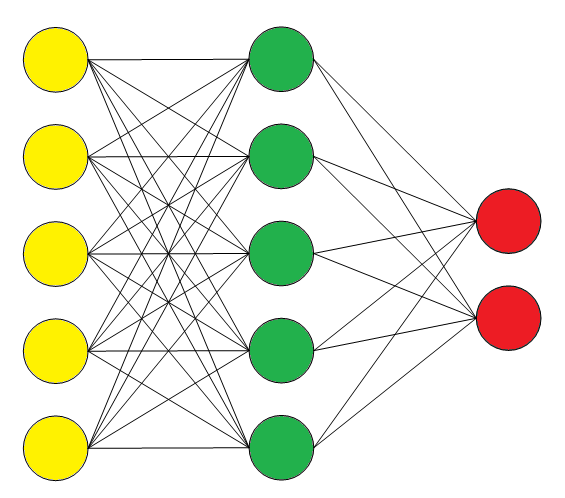
\includegraphics[width=0.5\textwidth]{images/ann.png}
			\end{center}
		\end{minipage}	
		\begin{minipage}[c]{0.48\textwidth}
			\begin{center}
			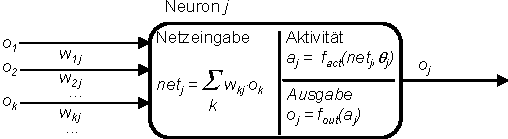
\includegraphics[width=\textwidth]{images/Neuron}
			\end{center}				
		\end{minipage}
		\begin{flushright}
			\tiny{[Quelle: Lehr- und Übungsbuch künstliche Intelligenz; Lämmel, Cleve; 2012]}
		\end{flushright}
	\end{frame}

	%!TEX root = abschlusspraesentation.tex

\begin{frame}[c]\frametitle{NN Auswertung}
\usetikzlibrary{arrows}
\usetikzlibrary{positioning} 
\usetikzlibrary{automata} 

  \def\wOne{{1.0,2.0,3.0,4.0}}
  \def\wTwo{{2.0,1.0,4.0,2.0,3.0,1.0}}

  \def\wOneAdjusted{{0.9,2.2,2.7,3.6}}
  \def\wTwoAdjusted{{3.0,0.5,3.7,1.8,2.5,0.5}}

  \def\inputValues{{0.3,0.2,0.5,0.6}}
  \def\results{{0.3,0.4,1.5,2.4}}
  \def\allresults{{-2.0, 4.6, 5.7, -3.0, 1.0, 4.4}}
  \def\allresultstransfered{{0.4, 0.8, 0.9, 0.3, 0.55, 0.8}}
  
  \def\rightresults{{0.3,0.4,1.5,2.4,2.0,2.0}}
  \def\allrightresults{{-5.7, 4.6, -5.7}}
  \def\allrightresultstransfered{{0.1, 0.8, 0.1}}
  \def\error{{-0.1, 0.2, -0.1}}
  \def\deltasoutput{{-0.0, 0.0, -0.0}}
  \def\deltashidden{{0.0, 0.0, 0.0, 0.0, 0.0, 0.0}}

  \begin{tikzpicture}[->,shorten >=1pt,auto, node distance=1cm, scale=0.9,
    thick,main node/.style={circle,fill=blue!20,draw,font=\sffamily\small\bfseries}]
    % =======
    % empty invisible node to avoid resize
    % =======
      \node at (-2,7) {};
    % =======
    % Input Neurons   
    % =======
    \only<1>{
      \foreach \x in {0, ..., 3} {
        \node[main node] (\x) at (0,5.8-1.2*\x) {};
      }
    }
    \only<2->{
      \foreach \x in {0, ..., 3} {
        \node[main node] (\x) at (0,5.8-1.2*\x) {$\pgfmathparse{\inputValues[\x}\pgfmathresult$};
      }
    }


    % =======
    % Hidden Neurons   
    % =======
    \only<1-3> {
      \foreach \x in {0, ..., 5} {
        \node[main node] (1\x) at (4,7-1.2*\x) {};
      }
    }
    \only<4> {
      \foreach \x in {0,2,3,4,5} {
        \node[main node] (1\x) at (4,7-1.2*\x) {};
      }
      \node[main node] (11) at (4,7-1.2) {$\pgfmathparse{\allresults[1}\pgfmathresult$};
    }
    \only<5> {
      \foreach \x in {0,...,5} {
        \node[main node] (1\x) at (4,7-1.2*\x) {$\pgfmathparse{\allresults[\x}\pgfmathresult$};
      }
    }
     \only<6-13> {
      \foreach \x in {0,...,5} {
        \node[main node] (1\x) at (4,7-1.2*\x) {$\pgfmathparse{\allresultstransfered[\x}\pgfmathresult$};
      }
    }
    \only<14-> {
      \foreach \x in {0,...,5} {
        \node[main node] (1\x) at (4,7-1.2*\x) {$\pgfmathparse{\deltashidden[\x}\pgfmathresult$};
      }
    }


    % =======
    % Output Neurons   
    % =======
    \only<1-7> {
      \foreach \x in {0, ..., 2} {
        \node[main node] (2\x) at (8,5.2-1.2*\x) {};
      }
    }
    \only<8> {
      \foreach \x in {0, 2} {
        \node[main node] (2\x) at (8,5.2-1.2*\x) {};
      }
       \node[main node] (21) at (8,5.2-1.2) {$\pgfmathparse{\allrightresults[1}\pgfmathresult$};
    }
     \only<9> {
      \foreach \x in {0,..., 2} {
        \node[main node] (2\x) at (8,5.2-1.2*\x) {$\pgfmathparse{\allrightresults[\x}\pgfmathresult$};
      }
       
    }
     \only<10> {
      \foreach \x in {0,..., 2} {
        \node[main node] (2\x) at (8,5.2-1.2*\x) {$\pgfmathparse{\allrightresultstransfered[\x}\pgfmathresult$};
      }
       
    }

    \only<11> {
      \foreach \x in {0,..., 2} {
          \node[main node] (2\x) at (8,5.2-1.2*\x) {$\pgfmathparse{\error[\x}\pgfmathresult$};
      }
    }
    \only<12-> {
      \foreach \x in {0,..., 2} {
          \node[main node] (2\x) at (8,5.2-1.2*\x) {$\pgfmathparse{\deltasoutput[\x}\pgfmathresult$};
      }
    }

    
    


    
    % \ifthenelse{\iStepTwo>0 \and \iStepTwo<11}{
    %   \foreach \x in {0, ..., 3} {
    %     \node at (0.1*\iStepTwo,5.8-1.2*\x+\iStepTwo*\x*0.06) {\pgfmathparse{\inputValues[\x}\pgfmathresult};
    %   }
    % } 

    % \ifthenelse{\iStepThree>0 \and \iStepThree<11}{
    %   \foreach \x in {0, ..., 3} {
    %     \node [opacity=1.0-0.1*\iStepThree] at (1.0+0.08*\iStepThree,5.8-0.6*\x) {\pgfmathparse{\inputValues[\x}\pgfmathresult};
    %   }
    % } 

    % \ifthenelse{\iStepFour>0 \and \iStepFour<11}{
    %   \foreach \x in {0, ..., 3} {
    %     \node [opacity=0.1*\iStepFour] at (1.8,5.8-0.6*\x) {\pgfmathparse{\results[\x}\pgfmathresult};
    %   }
    % } 

    % \ifthenelse{\iStepFive>0 \and \iStepFive<11}{
    %   \foreach \x in {0, ..., 3} {
    %     \node at (1.8+0.2*\iStepFive,5.8-0.6*\x+0.06*\iStepFive*\x) {\pgfmathparse{\results[\x}\pgfmathresult};
    %   }
    % } 
    
    % =======
    % edges   
    % ======= 
    \only<1> {
      \foreach \x in {0, ..., 3} 
        \foreach \y in {0, ..., 5} {
          \ifthenelse{\y=1}{
            \path[every node/.style={font=\sffamily\small}]
              (\x) edge [opacity=0.5] node [left] {} (1\y);
          }{
            \path[every node/.style={font=\sffamily\small}]
              (\x) edge [opacity=0.2] node [left] {} (1\y);
          }
        }
      
      \foreach \x in {0, ..., 5} 
        \foreach \y in {0, ..., 2} {
          \ifthenelse{\y=1}{
            \path[every node/.style={font=\sffamily\small}]
              (1\x) edge [opacity=0.5] node [left] {} (2\y);
          }{
            \path[every node/.style={font=\sffamily\small}]
              (1\x) edge [opacity=0.2] node [left] {} (2\y);
          }
        }
    }
    
    \only<2> {
      \foreach \x in {0, ..., 3} 
        \foreach \y in {0, ..., 5} {
          \ifthenelse{\y=1}{
            \path[every node/.style={font=\sffamily\small}]
              (\x) edge [opacity=0.5] node [left, sloped, above, opacity=1.0] {$\pgfmathparse{\wOne[\x}\pgfmathresult$} (1\y);
          }
        }
      
      \foreach \x in {0, ..., 5} 
        \foreach \y in {0, ..., 2} {
          \ifthenelse{\y=1}{
            \path[every node/.style={font=\sffamily\small}]
              (1\x) edge [opacity=0.5] node [left, sloped, above, opacity=1.0] {$\pgfmathparse{\wTwo[\x}\pgfmathresult$} (2\y);
          }
        }
    }

    \only<3> {
      \foreach \x in {0, ..., 3} 
        \foreach \y in {0, ..., 5} {
          \ifthenelse{\y=1}{
            \path[every node/.style={font=\sffamily\small}]
              (\x) edge [opacity=0.5] node [left, sloped, above, opacity=1.0, pos=0.4] {$\pgfmathparse{\inputValues[\x}\pgfmathresult\cdot\pgfmathparse{\wOne[\x}\pgfmathresult=\pgfmathparse{\results[\x}\pgfmathresult$} (1\y);
          }
        }
      
      \foreach \x in {0, ..., 5} 
        \foreach \y in {0, ..., 2} {
          \ifthenelse{\y=1}{
            \path[every node/.style={font=\sffamily\small}]
              (1\x) edge [opacity=0.5] node [left, sloped, above, opacity=1.0] {$\pgfmathparse{\wTwo[\x}\pgfmathresult$} (2\y);
          }
        }
    }

    \only<4-6> {
      \foreach \x in {0, ..., 3} 
        \foreach \y in {0, ..., 5} {
          \ifthenelse{\y=1}{
            \path[every node/.style={font=\sffamily\small}]
              (\x) edge [opacity=0.5] node [left, sloped, above, opacity=1.0, pos=0.4] {$\pgfmathparse{\wOne[\x}\pgfmathresult$} (1\y);
          }
        }
      
      \foreach \x in {0, ..., 5} 
        \foreach \y in {0, ..., 2} {
          \ifthenelse{\y=1}{
            \path[every node/.style={font=\sffamily\small}]
              (1\x) edge [opacity=0.5] node [left, sloped, above, opacity=1.0] {$\pgfmathparse{\wTwo[\x}\pgfmathresult$} (2\y);
          }
        }
    }
    \only<7> {
      \foreach \x in {0, ..., 3} 
        \foreach \y in {0, ..., 5} {
          \ifthenelse{\y=1}{
            \path[every node/.style={font=\sffamily\small}]
              (\x) edge [opacity=0.5] node [left, sloped, above, opacity=1.0, pos=0.4] {$\pgfmathparse{\wOne[\x}\pgfmathresult$} (1\y);
          }
        }
      
      \foreach \x in {0, ..., 5} 
        \foreach \y in {0, ..., 2} {
          \ifthenelse{\y=1}{
            \path[every node/.style={font=\sffamily\small}]
              (1\x) edge [opacity=0.5] node [left, sloped, above, opacity=1.0, pos=0.4] {$\pgfmathparse{\allresultstransfered[\x}\pgfmathresult\cdot\pgfmathparse{\wTwo[\x}\pgfmathresult=\pgfmathparse{\rightresults[\x}\pgfmathresult$} (2\y);
          }
        }
    }
    \only<8-12> {
      \foreach \x in {0, ..., 3} 
        \foreach \y in {0, ..., 5} {
          \ifthenelse{\y=1}{
            \path[every node/.style={font=\sffamily\small}]
              (\x) edge [opacity=0.5] node [left, sloped, above, opacity=1.0, pos=0.4] {$\pgfmathparse{\wOne[\x}\pgfmathresult$} (1\y);
          }
        }
      
      \foreach \x in {0, ..., 5} 
        \foreach \y in {0, ..., 2} {
          \ifthenelse{\y=1}{
            \path[every node/.style={font=\sffamily\small}]
              (1\x) edge [opacity=0.5] node [left, sloped, above, opacity=1.0] {$\pgfmathparse{\wTwo[\x}\pgfmathresult$} (2\y);
          }
        }
    }
    \only<13-14> {
      \foreach \x in {0, ..., 3} 
        \foreach \y in {0, ..., 5} {
          \ifthenelse{\y=1}{
            \path[every node/.style={font=\sffamily\small}]
              (\x) edge [opacity=0.5] node [left, sloped, above, opacity=1.0, pos=0.4] {$\pgfmathparse{\wOne[\x}\pgfmathresult$} (1\y);
          }
        }
      
      \foreach \x in {0, ..., 5} 
        \foreach \y in {0, ..., 2} {
          \ifthenelse{\y=1}{
            \path[every node/.style={font=\sffamily\small}]
              (1\x) edge [opacity=0.5] node [left, sloped, above, opacity=1.0] {$\pgfmathparse{\wTwoAdjusted[\x}\pgfmathresult$} (2\y);
          }
        }
    }
    \only<15-> {
      \foreach \x in {0, ..., 3} 
        \foreach \y in {0, ..., 5} {
          \ifthenelse{\y=1}{
            \path[every node/.style={font=\sffamily\small}]
              (\x) edge [opacity=0.5] node [left, sloped, above, opacity=1.0, pos=0.4] {$\pgfmathparse{\wOneAdjusted[\x}\pgfmathresult$} (1\y);
          }
        }
      
      \foreach \x in {0, ..., 5} 
        \foreach \y in {0, ..., 2} {
          \ifthenelse{\y=1}{
            \path[every node/.style={font=\sffamily\small}]
              (1\x) edge [opacity=0.5] node [left, sloped, above, opacity=1.0] {$\pgfmathparse{\wTwoAdjusted[\x}\pgfmathresult$} (2\y);
          }
        }
    }
   \end{tikzpicture}
  \begin{itemize}
    \only<1> {
      \item Multilayerperceptron-Netz
    }
    \only<2> {
      \item Trainingseingabe und Kantengewichte
    }
    \only<3> {
      \item Gewichtung der Trainingseingabe mit Kantengewicht
    }
    \only<4> {
      \item Summe der Produkte ergibt Netzeingabe in der Hidden-Schicht
    }
    \only<5> {
      \item Netzeingabe der restlichen Neuronen der Hidden-Schicht
    }
    \only<6> {
      \item Umrechnung der Netzeingabe mit der Übertragungsfunktion (sigmoiddelta)
    }
    \only<7> {
      \item Gewichtung der Ausgabewerte mit Kantengewicht
    }
    \only<8> {
      \item Summe der Produkte ergibt Netzeingabe in der Ausgabeschicht
    }
    \only<9> {
      \item Netzeingabe der restlichen Neuronen der Ausgabeschicht
    }
    \only<10> {
      \item Umrechnung der Netzeingabe mit der Übertragungsfunktion (sigmoiddelta)
    }
    \only<11> {
      \item Berechnung des Ausgabefehlers anhand Ausgabewert und gewünschtem Ausgabewert
    }
    \only<12> {
      \item Berechnung von delta-Werten anhand Netzeingabe, Übertragungsfunktion und Ausgabefehler 
    }
    \only<13> {
      \item Anpassung der Kantengewichte
    }
    \only<14> {
      \item Berechnung von delta-Werten in Hidden-Schicht (benötigt u.a. ausgehende Kantengewichte und delta-Werte der Ausgabeschicht)
    }
    \only<15> {
      \item Anpassung der Kantengewichte
    }
   \end{itemize}
  
% \item<1> Multilayerperceptron-Netz
%       \item<2> Trainingseingabe und Kantengewichte
%       \item<3> Gewichtung der Trainingseingabe mit Kantengewicht
%       \item<4> Summe der Produkte ergibt Netzeingabe in der Hidden-Schicht
%       \item<5> Netzeingabe der restlichen Neuronen der Hidden-Schicht
%       \item<6> Umrechnung der Netzeingabe mit der Übertragungsfunktion (sigmoiddelta)
%       \item<7> Gewichtung der Ausgabewerte mit Kantengewicht
%       \item<8> Summe der Produkte ergibt Netzeingabe in der Output-Schicht
%       \item<9> Netzeingabe der restlichen Neuronen der Output-Schicht
%       \item<10> Umrechnung der Netzeingabe mit der Übertragungsfunktion (sigmoiddelta)
%       \item<11> b
%       \item<12> Berechnung von delta-Werten anhand Netzeingabe, Übertragungsfunktion und Ausgabefehler 
%       \item<13> b

    % \node[main node] (0) {5};
    % \node[main node] (1) [below of=0] {\only<2>{test}};
    % \node[main node] (2) [below of=1] {3};
    % \node[main node] (3) [below of=2] {4};

    % \node[main node] (11) [right of=0] {2};
    % \node[main node] (10) [above of=11] {2};
    % \node[main node] (12) [right of=1] {2};
    % \node[main node] (13) [right of=2] {2};
    % \node[main node] (14) [right of=3] {2};
    % \node[main node] (15) [below of=14] {2};

    % \node[main node] (20) [below right  of=10] {2};
    % \node[main node] (21) [below right  of=12] {2};
    % \node[main node] (22) [below right  of=14] {2};

    % \path[every node/.style={font=\sffamily\small}]
    %   (0) edge node [left] {0.6} (10)
    %       edge node[left] {0.3} (11)
    %       edge node {0.1} (12)
    %   (1) edge node [right] {0.4} (10)
    %       edge node {0.3} (11)
    %       edge node {0.4} (12)
    %       edge node {0.1} (13)
    %   (2) edge node [right] {0.8} (13)
    %       edge node [right] {0.2} (14)
    %       edge node [right] {0.2} (15)
    %   (3) edge node [left] {0.2} (15)

    %   (10)edge node [left] {0.6} (20)
    %   (11)edge node [right] {0.4} (20)
    %       edge node {0.3} (21)
    %       edge node {0.4} (22)
    %   (12)edge node [right] {0.8} (21)
    %       edge node [right] {0.2} (20)
    %   (13)edge node [left] {0.2} (20)
    %   (14)edge node [right] {0.8} (21)
    %       edge node [right] {0.2} (22)
    %   ;
    
\end{frame}
	

	\begin{frame}[c]\frametitle{Neuronale Netze}
		\begin{center}
		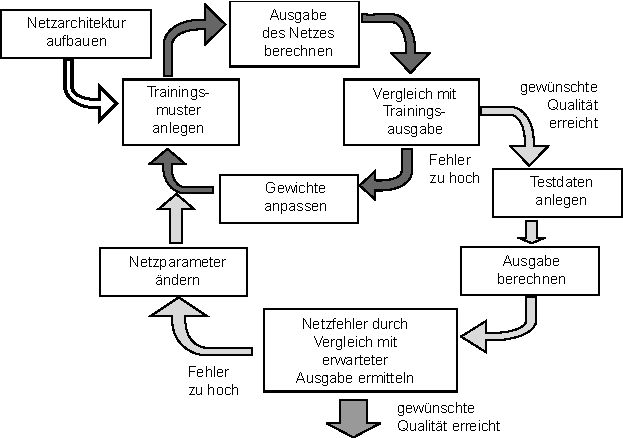
\includegraphics[scale=.8]{images/workflow}
		\end{center}
		\begin{flushright}
		\tiny{[Quelle: Lehr- und Übungsbuch künstliche Intelligenz; Lämmel, Cleve; 2012]}
		\end{flushright}
	\end{frame}	
	
	\subsection{Simulationsumgebung Neuroph}
	\begin{frame}[c]\frametitle{Neuroph}
		\begin{itemize}
		\item Simulationsumgebung für Neuronale Netze
		\item 42751 LOC
		\item Apache 2.0 Lizenz
		\item \url{http://neuroph.sourceforge.net/}
		\end{itemize}
		\begin{center}
		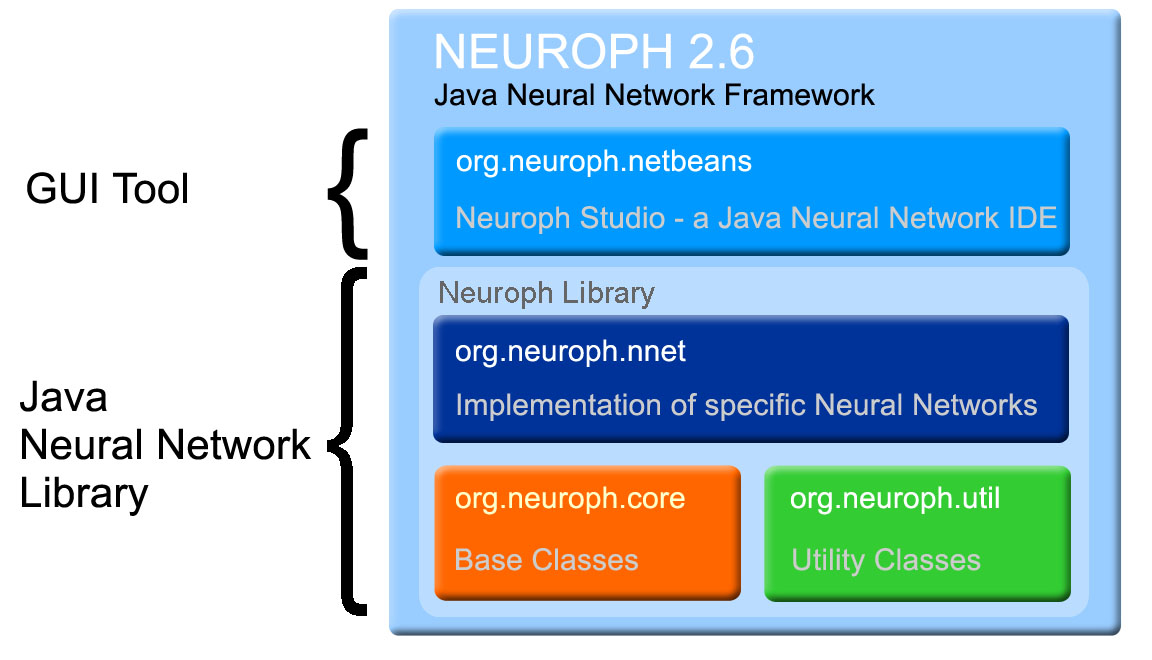
\includegraphics[width=.75\textwidth]{Grafiken/NeurophFrameworkDiagram.jpg} 
		\end{center}
	\end{frame}	
	
	\subsection{Überblick}
	\begin{frame}[c]\frametitle{Überblick}
  		\begin{gantt}[xunitlength=1.75cm, fontsize=\tiny, titlefontsize=\tiny, drawledgerline=true]{10}{5}
    		\begin{ganttitle}
      			\titleelement{Okt. '12}{1}
      			\titleelement{Nov. '12}{1}
      			\titleelement{Dez. '12}{1}
      			\titleelement{Jan. '13}{1}
      			\titleelement{Feb. '13}{1}
    		\end{ganttitle}
    		\ganttbar{Themenfindung}{0}{1.2}
    		\ganttbar{Einarbeitung Neuronale Netze}{1}{2}
    		\ganttmilestone[color=cyan]{Themenvorstellung}{1.2}
    		\ganttbar{Code Analyse \& Profiling}{1}{1.5}
    		\ganttbar{Drei Parallelisierungsansätze}{1.6}{2}
    		\ganttmilestone[color=cyan]{Zwischenpräsentation}{3.23}
    		\ganttbar{Testdaten beschaffen}{2}{.5}
    		\ganttbarcon{Evaluierung der Ansätze}{2.5}{1.95}    		
    		\ganttmilestone[color=cyan]{Abschlusspräsentation}{4.45}     		
  		\end{gantt}
	\end{frame}	
	
	\begin{frame}[c]\frametitle{Überblick}
		\begin{itemize}
		   \item Einleitung \checkmark
		   \item Neuroph auf Code-Ebene 
		   \item Drei Parallelisierungsansätze
		   \item Evaluierung
		   \item Fazit
		\end{itemize}
	\end{frame}
	
	\section{Neuroph auf Code-Ebene}
	\subsection{Neuroph auf Code-Ebene}
	\begin{frame}[c]\frametitle{Code Analyse}
		\begin{block}{Was wir vorgefunden haben}
			\begin{center}
				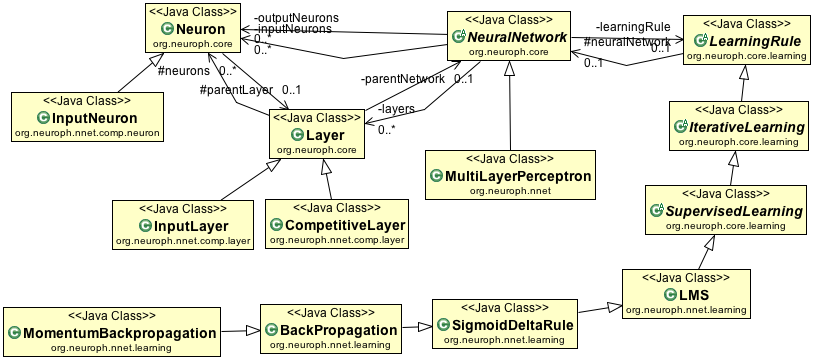
\includegraphics[scale=0.4]{images/Klassendiagramm.png}
			\end{center}
		\end{block}
	\end{frame}
	
	\begin{frame}[c]\frametitle{Code Analyse: Sequenzdiagramm}
			\begin{center}
			  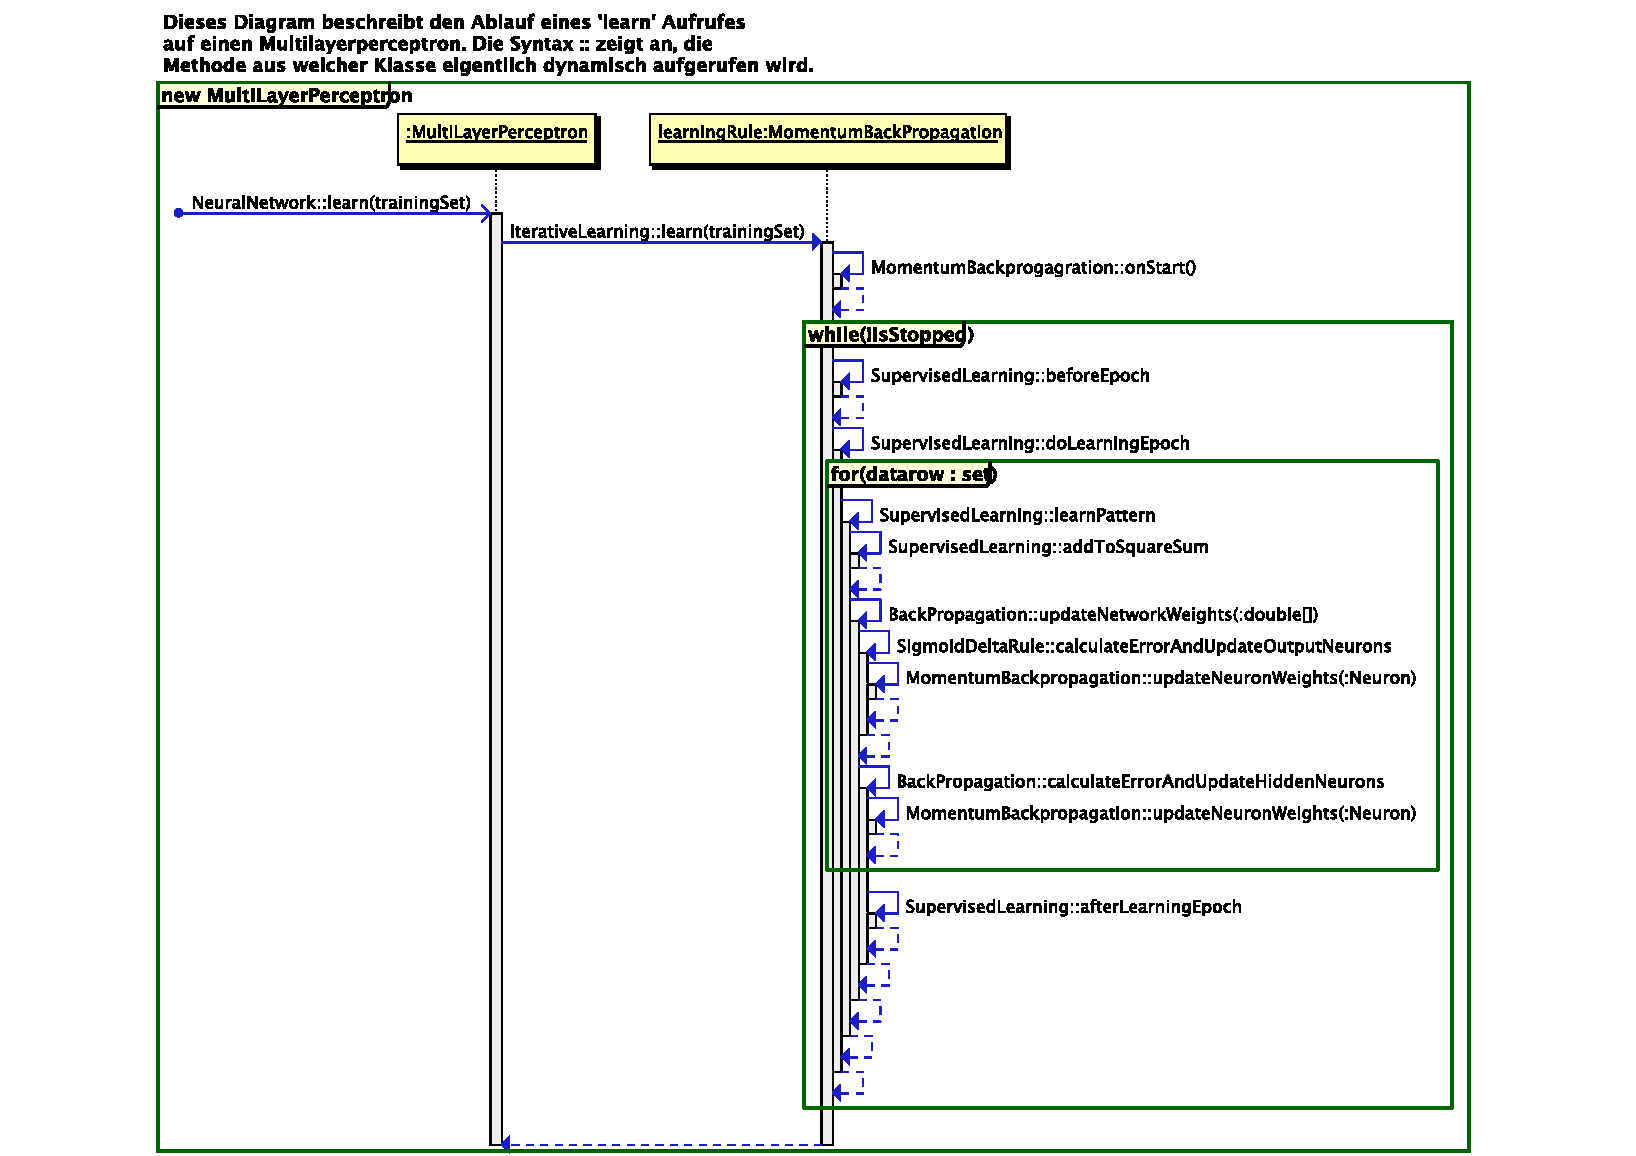
\includegraphics[scale=0.4]{images/Learn.pdf} 
			\end{center}
	\end {frame}			
	
	\section{Parallelisierungsansätze}
	\begin{frame}[c]\frametitle{Parallelisierungsansätze}
		\begin{itemize}
			\item Layer-Partitionierung
			\item Batch Learning Parallelisierung
			\item Clonebased Parallelisierung
		\end{itemize}	
	\end{frame}
	
	\subsection{Layer-Partitionierung}
	\begin{frame}[c, fragile, allowframebreaks]\frametitle{Layer-Partitionierung}
	    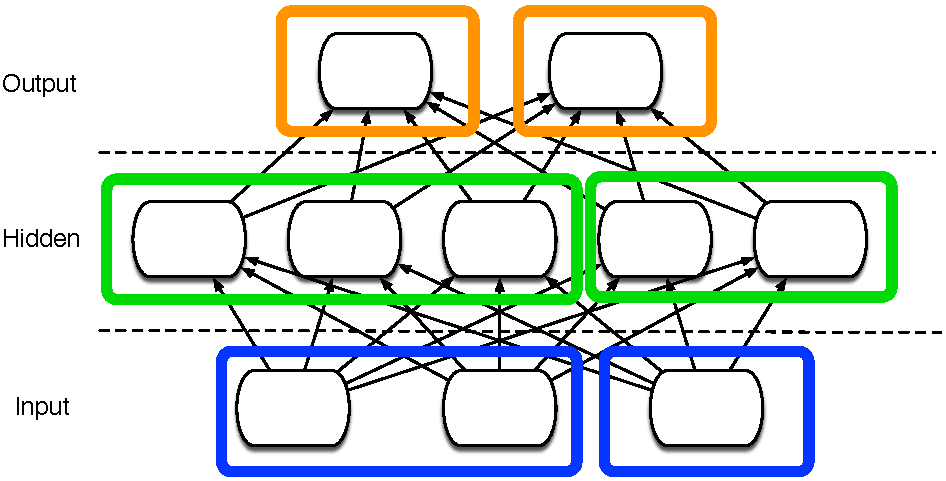
\includegraphics[scale=0.7]{Grafiken/Feingranular.pdf}
	
	\framebreak

		\begin{block}{Layer::calculate()}
			\begin{lstlisting}
			for (Neuron n : this.neurons) 
			    n.calculate();
	 		\end{lstlisting}
 		\end{block}

		\begin{block}{ParallelLayer::calculate()}
	 		\begin{lstlisting}
			ExecutorService service = getExecutor();
			Queue<Future<?>> futures = new LinkedList<>();

			for (NeuronJob j : jobs)
			    futures.add(service.submit(j));
			
			waitForAll(futures);
	 		\end{lstlisting}
	 	\end{block}

 		\framebreak
	
		\begin{itemize}
			\item Neuer Netzwerktyp: Paralleles neurales Netzwerk
			\item Zu feingranular, Concurrency-Overhead überwiegt erhoffte Zeitersparnis
			\item Erster naiver Ansatz $\rightarrow$ gescheitert!		
			% TODO Zahlen hier einfügen			
		\end{itemize}	
		\begin{center}
			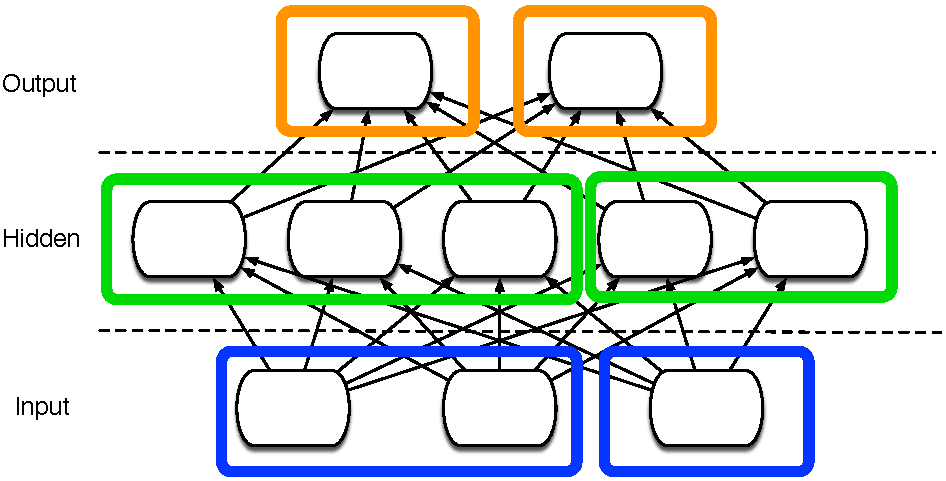
\includegraphics[scale=0.25]{Grafiken/Feingranular.pdf}
		\end{center}
	\end{frame}
	
	\subsection{Batch Parallelisierung}
	\begin{frame}[c]\frametitle{Exkurs: Batch lernen}
		\begin{center}
			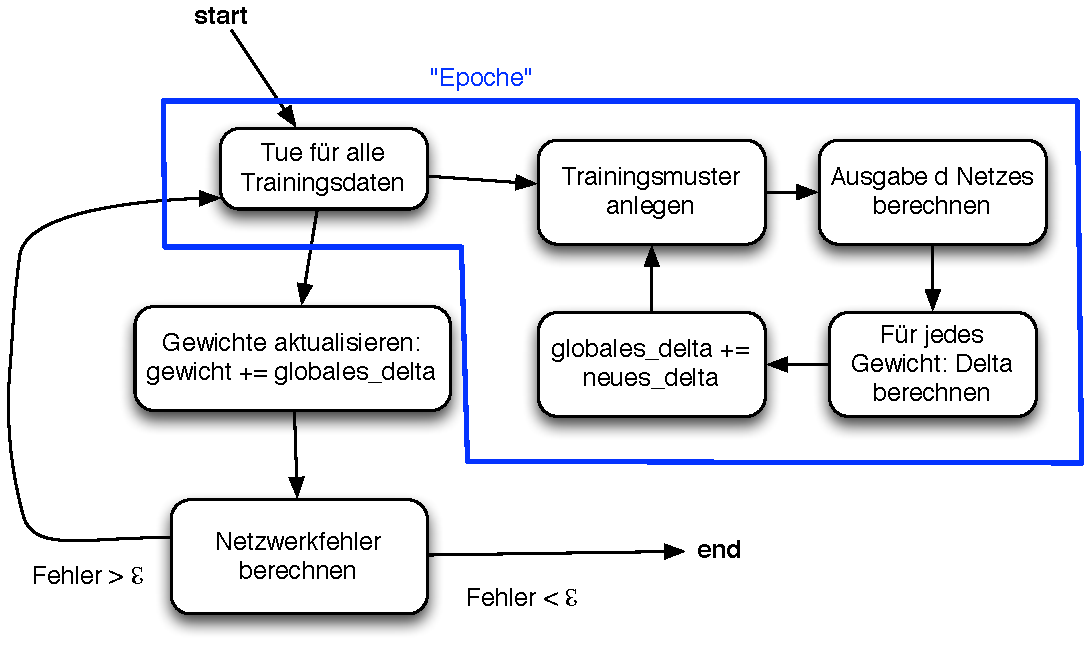
\includegraphics[scale=0.6]{Grafiken/Batchlearning.pdf}		    
		\end{center}	
	\end{frame}

	\begin{frame}[c,allowframebreaks]\frametitle{Batch Learning Parallelisierung}

		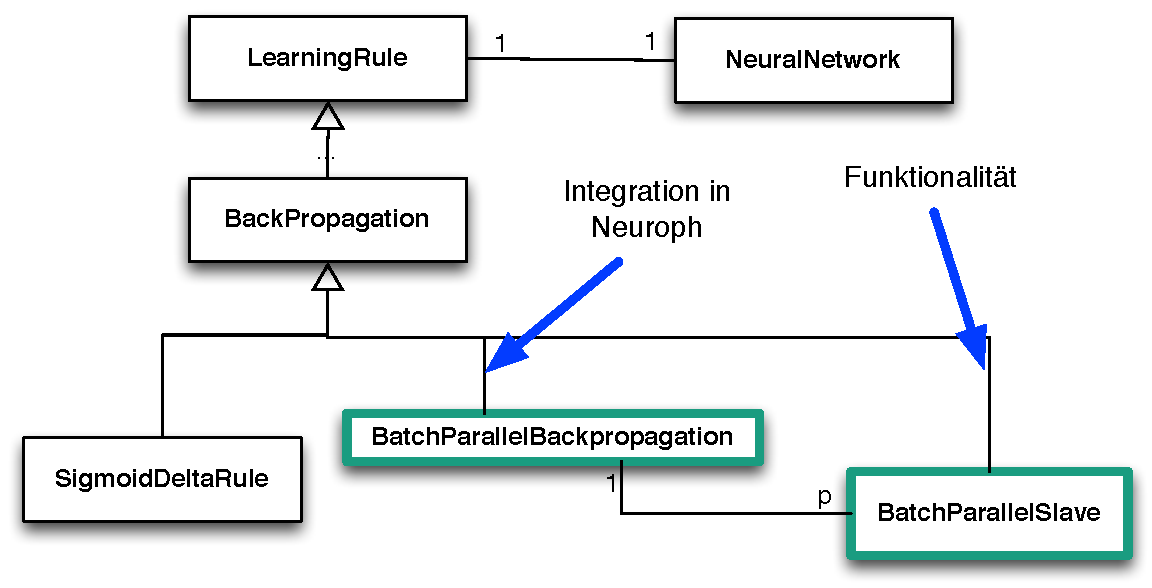
\includegraphics[scale=0.58]{Grafiken/Batchparallel_uml.pdf}
		\\
		\textbf{\textit{Paralleles Lernen statt parallelem Netzwerk}}
	\framebreak

		\begin{itemize}
			\item Paralleler Lernvorgang (Netzwerk sequentiell)
			\item Vorteil:
			\begin{itemize}
				\item Saubere, konsistente Schnittstelle
				\item Zugriff auf \textit{protected} Funktionalität
			\end{itemize}
			\item Nachteil: 
			\begin{itemize}
				\item Lernalgorithmus fest 
				\begin{itemize}
					\item Backpropagation
				\end{itemize}
				\item Softwaretechnisch fragwürdig
				\begin{itemize}
					\item Beispiel: Override mit leerem Body
				\end{itemize}
			\end{itemize}
		\end{itemize}


	\framebreak

		\begin{itemize}
			\item Trainingsdaten auf Worker verteilt
			\item Worker lernen unabhängig
			\item Gewichtänderungen aufaddieren
			\begin{itemize}
				\item Jeder Thread bearbeitet Subset
				\item Dadurch keine Abhängigkeiten
			\end{itemize}
		\end{itemize}

	\framebreak
		\begin{center}
			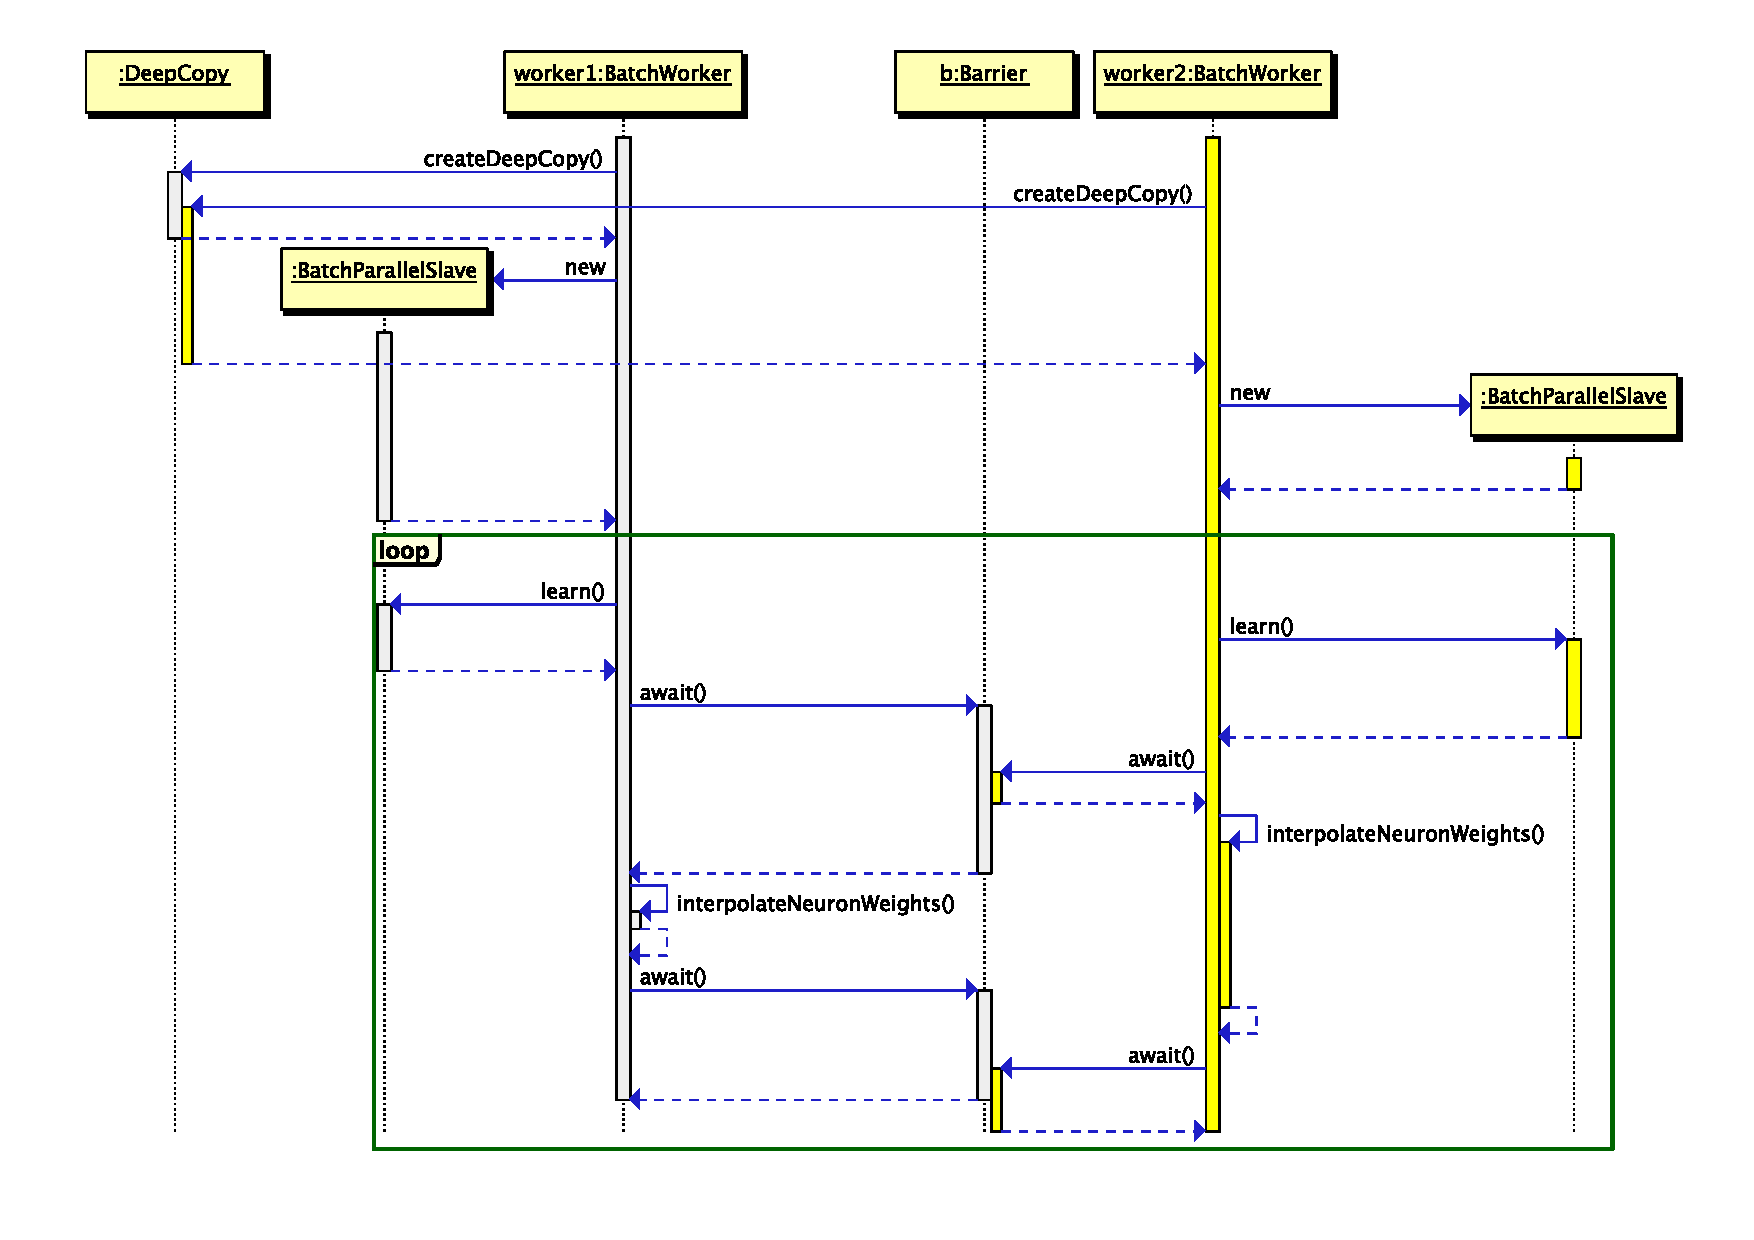
\includegraphics[scale=0.33]{Grafiken/Batch_seq.pdf}
		\end{center}

	\end{frame}
	
	\subsection{Clonebased Parallelisierung}
	\begin{frame}[allowframebreaks]{Clonebased Parallelisierung}
		\begin{block}{Charakteristika}
			\begin{itemize}
				\item Container für ein neuronales Netz mit überwachter Lernmethodik
				\item Unterteilt Trainingssatz und erlernt diese Teile parallel
				\item Abweichende Ergebnisgewichte verglichen mit sequentiellem Lernen
			\end{itemize}
		\end{block}
	
	\framebreak
		\begin{block}{Vorgehen}
			\begin{enumerate}
				\item Aufteilung des Trainingssatzes auf Worker-Threads
				\item Jeder Worker klont sich das Original-Netz
				\item Jeder Worker lernt eine Iteration
				\item Gewichts-Interpolation unter allen Worker-Klonnetzen
				\item $goto\ (3)$ bis maximale Iteration erreicht oder Fehler klein genug
			\end{enumerate}
		\end{block}
	
	\framebreak
		\begin{center}
			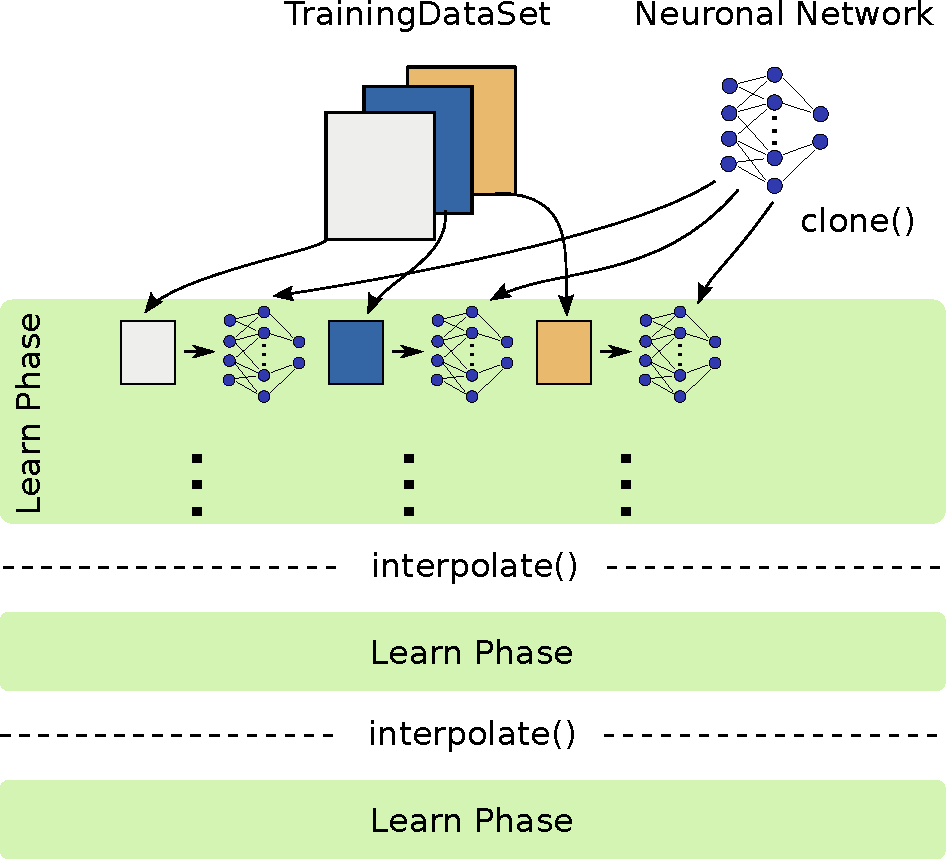
\includegraphics[width=.65\textwidth]{images/Parallelisierungsansatz.pdf} 
		\end{center}
	
	\framebreak
		\begin{block}{Interpolationstypen}
			$w = f(w_1,w_2,w_3,...,w_n)$
			\newline
			Gesucht: gute Interpolationsfunktion $f$
			\newline
			\newline
			\emph{Kandidaten:}
			\begin{itemize}
				\item Arithmetisches Mittel
				\item Minimum, Maximum
				\item Bestes bisheriges Gewicht \emph{("Genetischer Ansatz")}
			\end{itemize}
		\end{block}
		
	\framebreak
		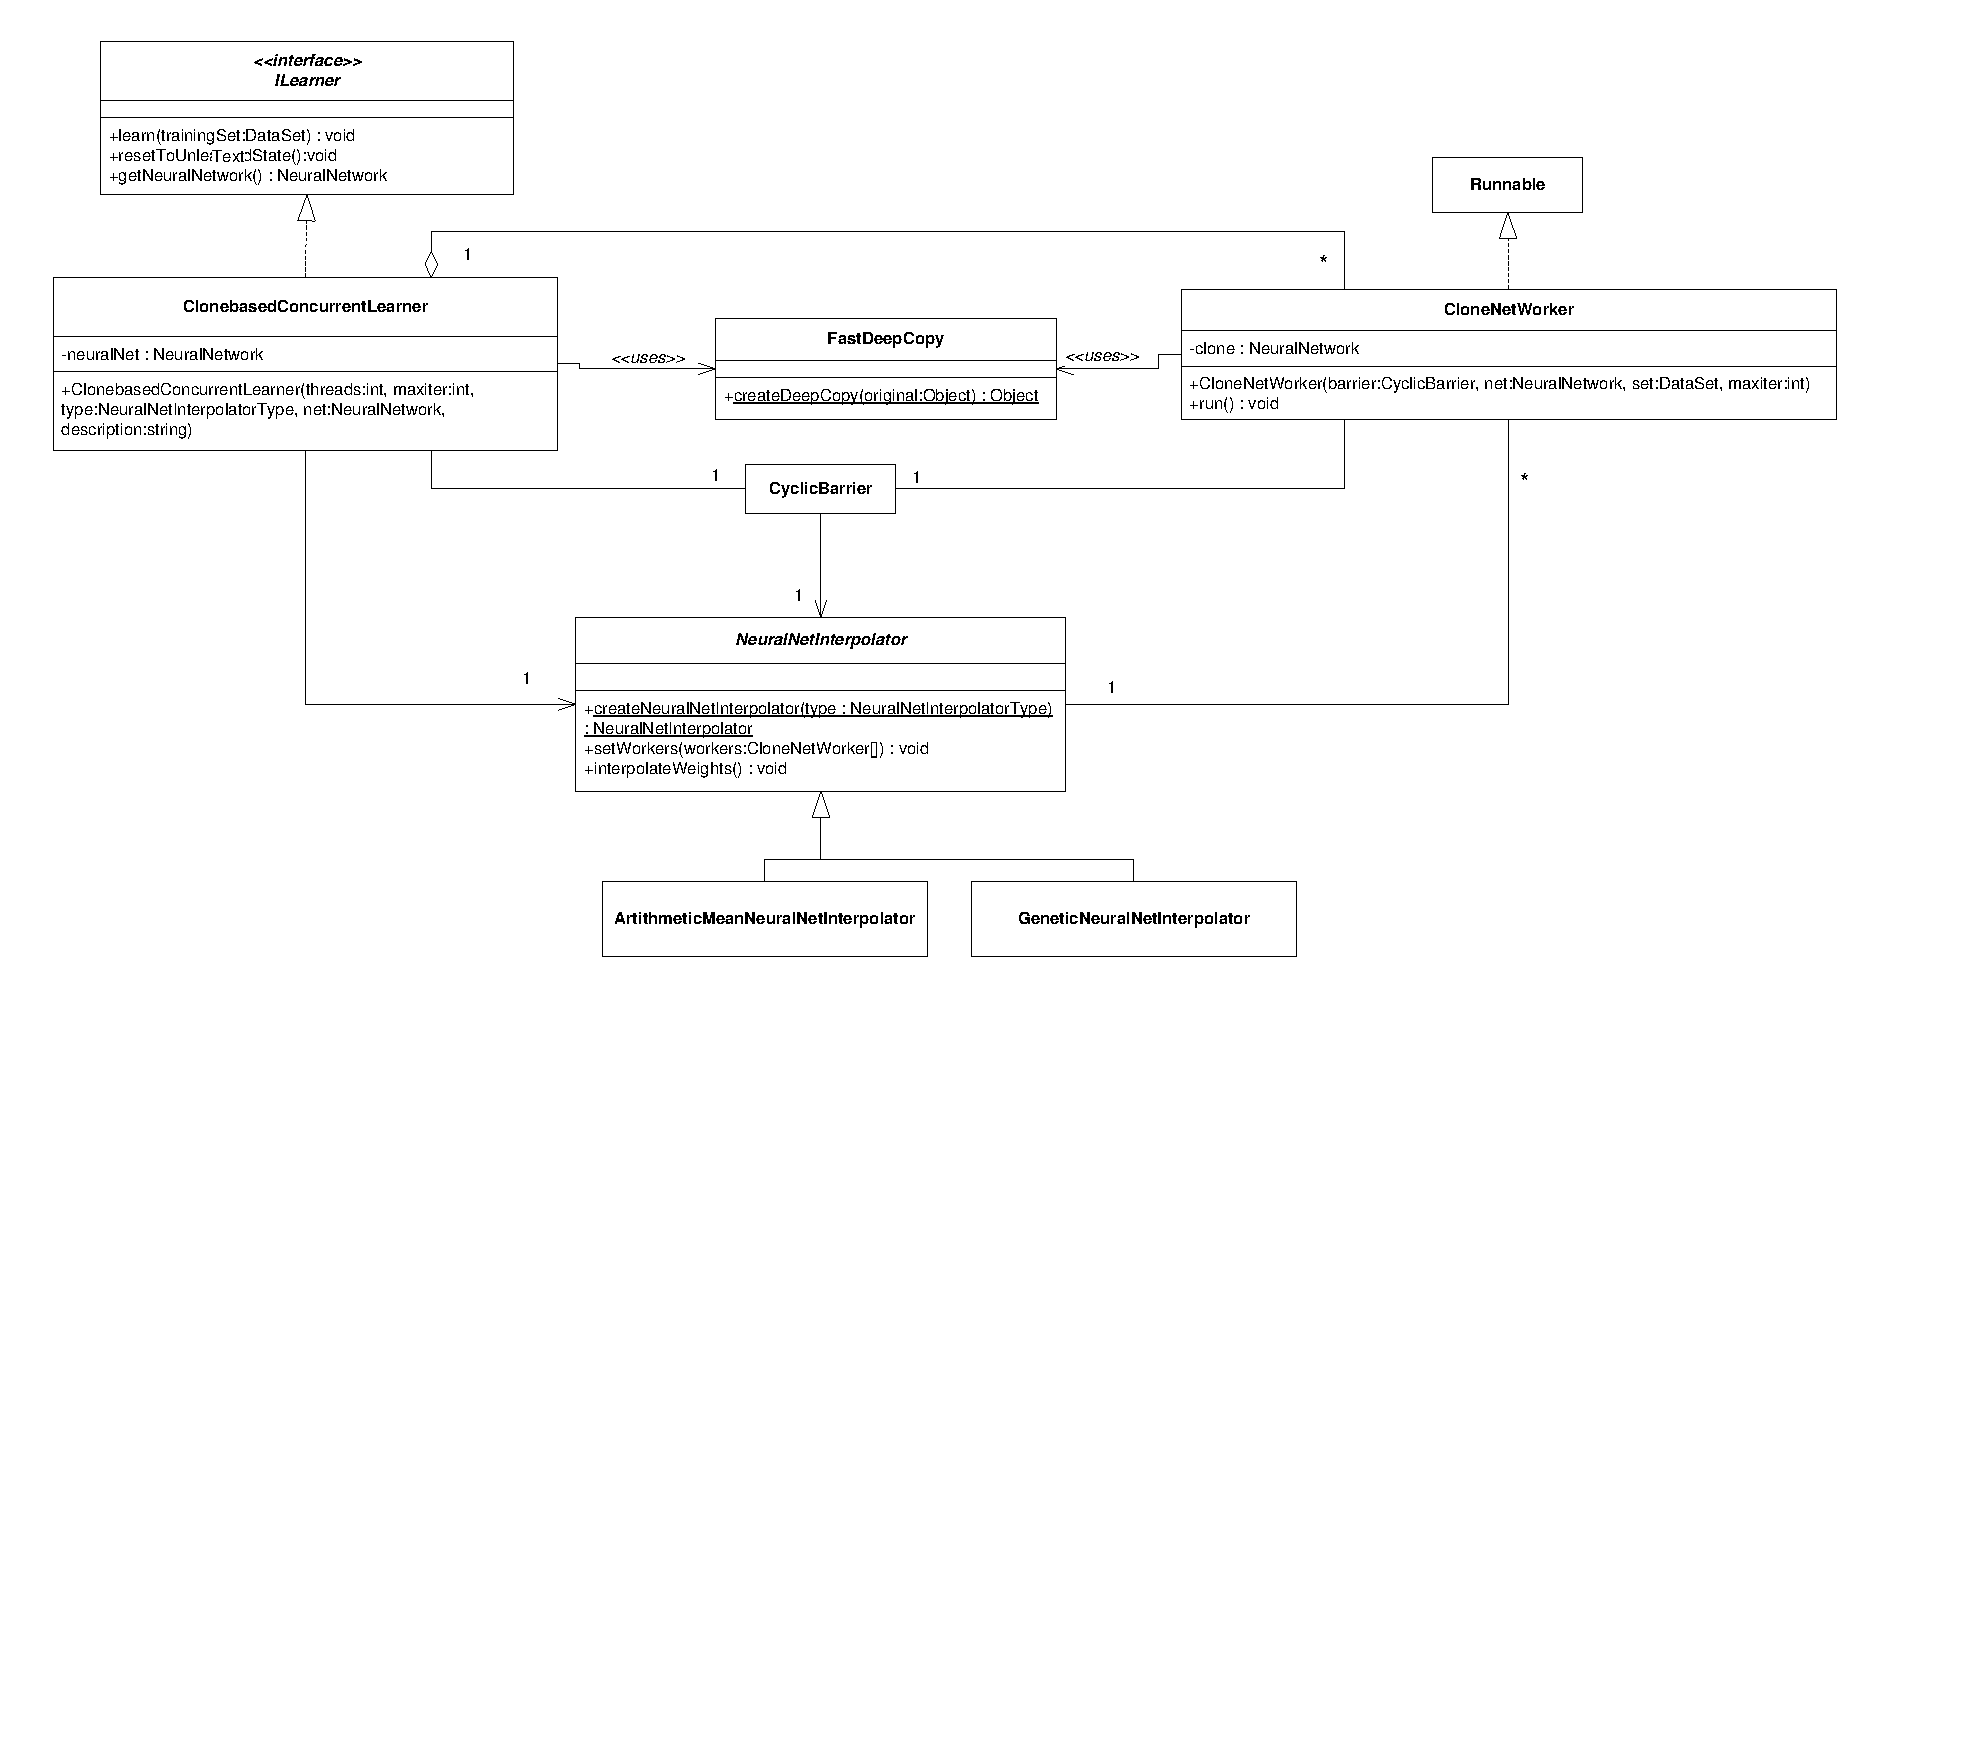
\includegraphics[height=0.8\textheight]{Grafiken/Clonebased_classdiagram}
		
	\framebreak
		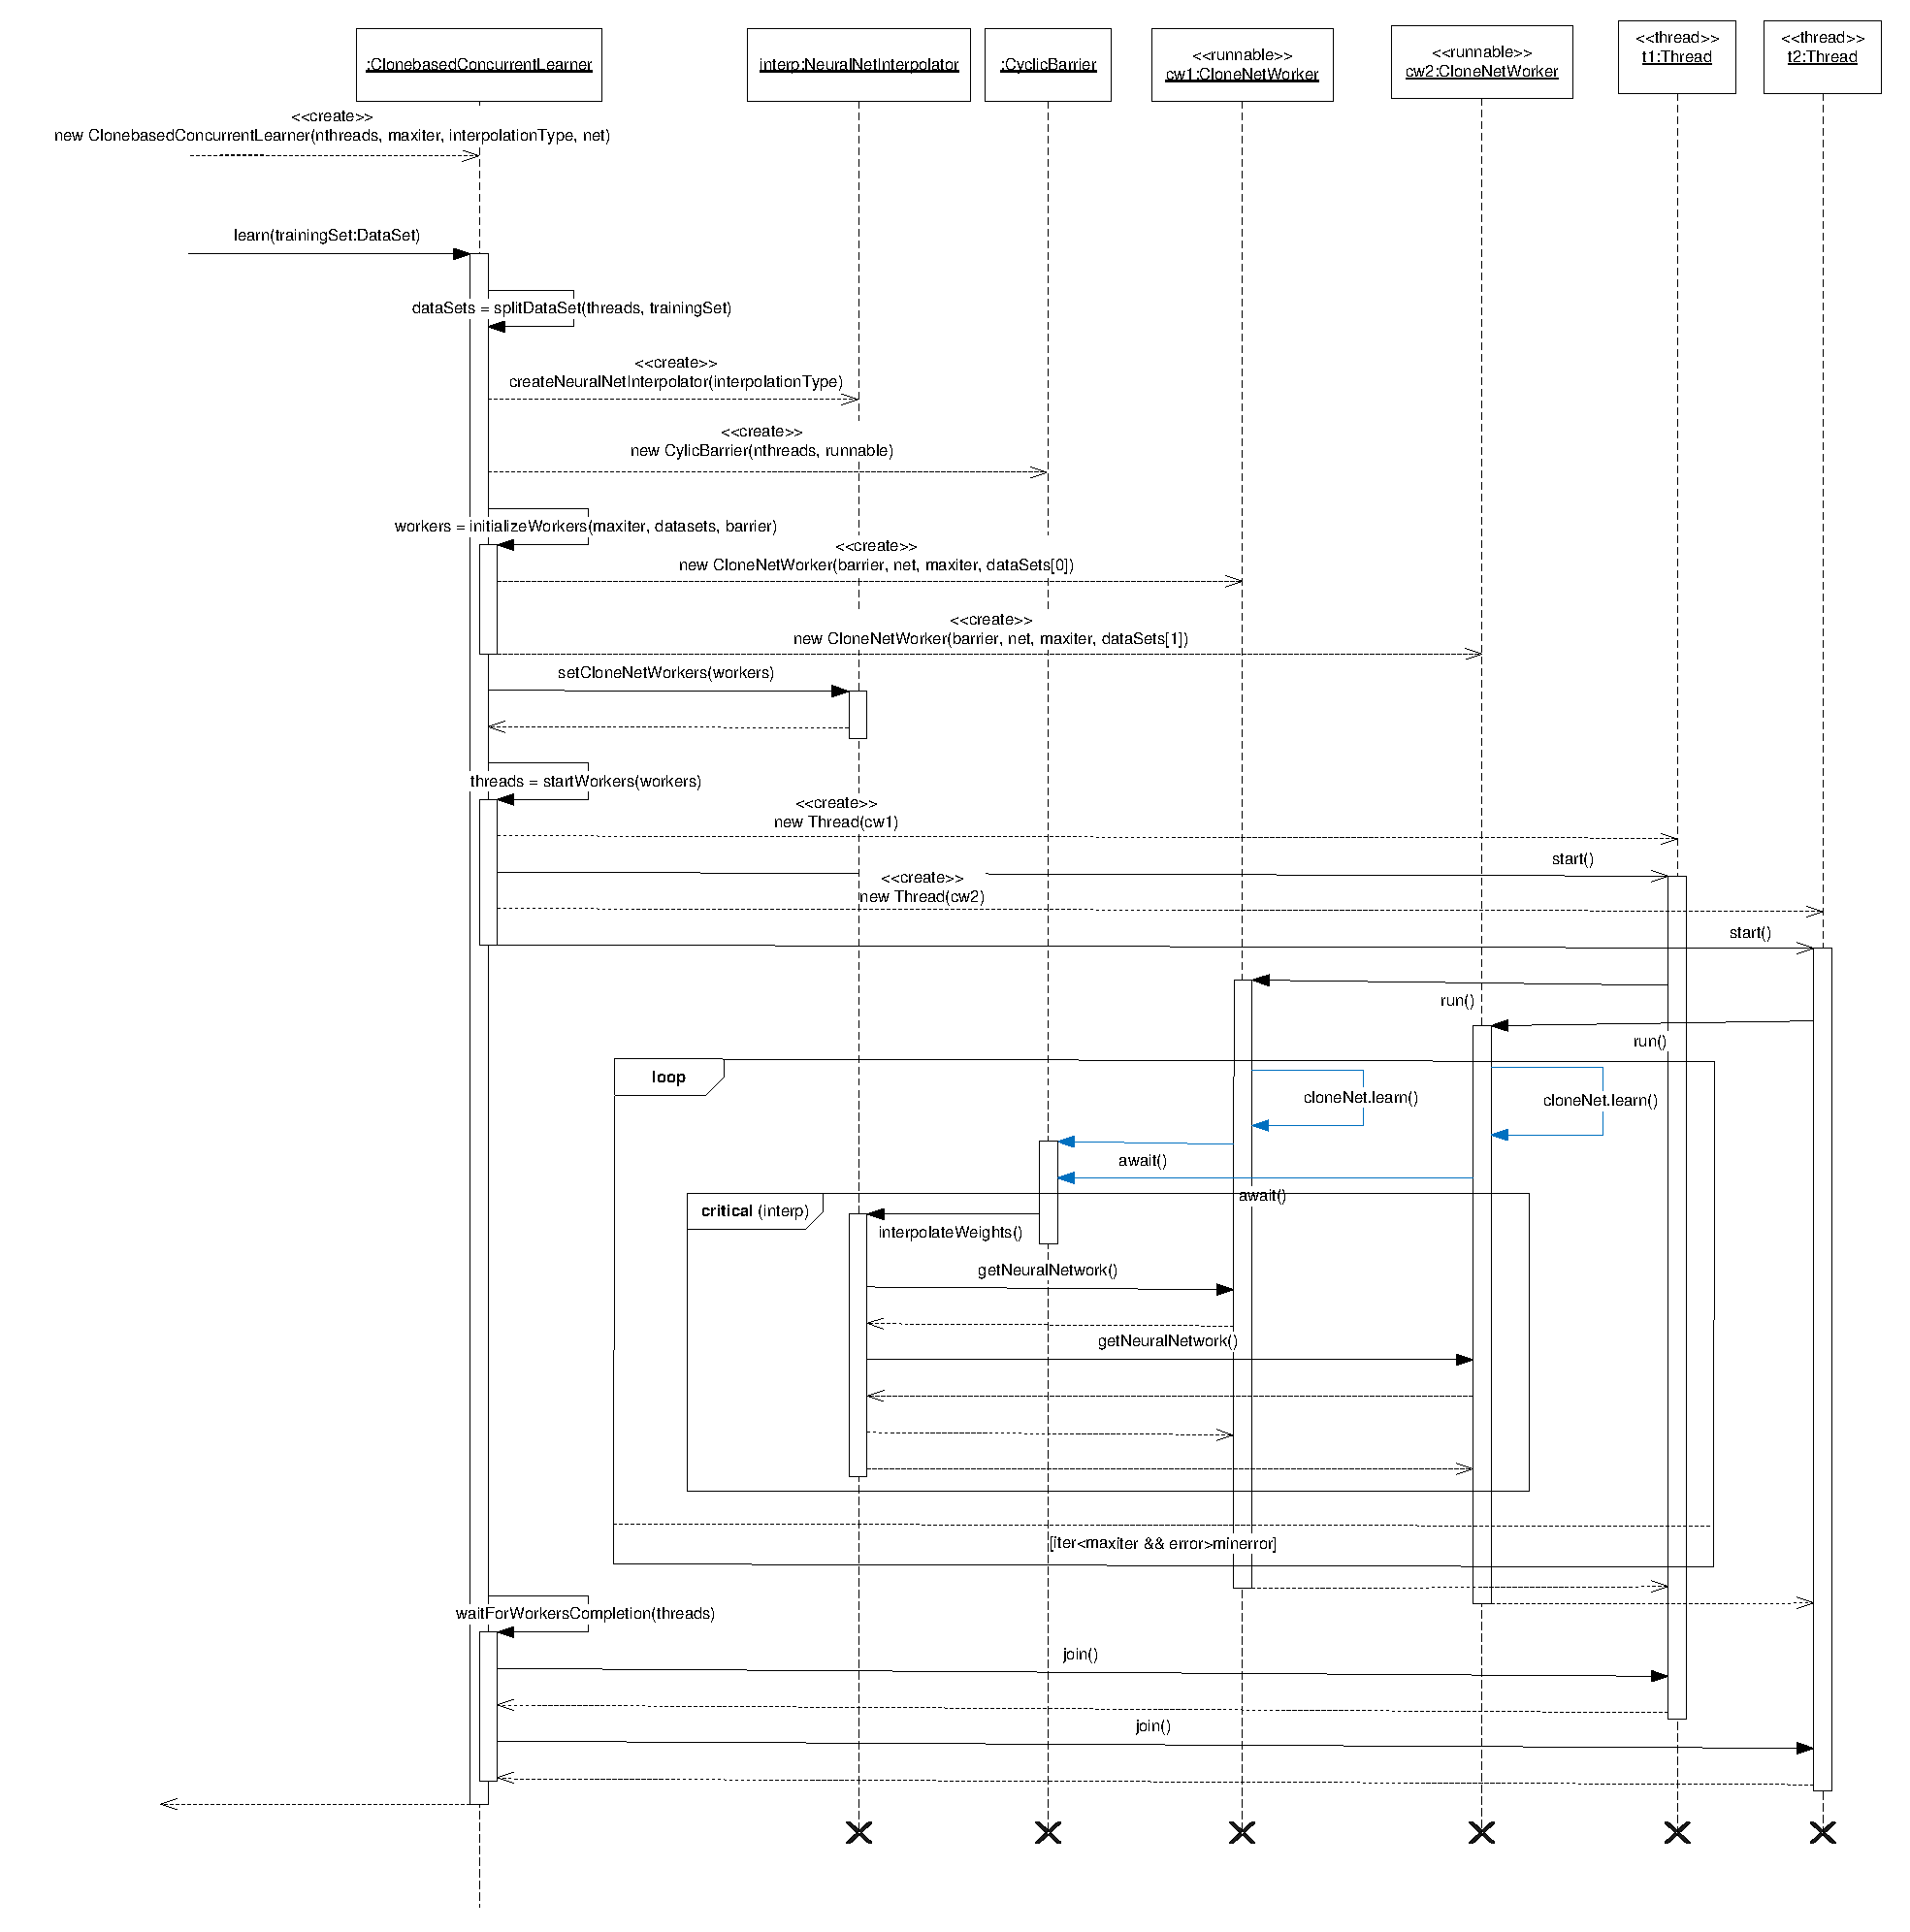
\includegraphics[height=0.8\textheight]{Grafiken/Clonebased_sequencediagram}
	\end{frame}

	\begin{frame}[c]\frametitle{Technischer Vergleich der Strategien}	
		\begin{tabular}{l|c|c|c|}

		Kategorie & Layerpartitionierung & Batch & Clonebased \\
		\hline
		Was ist parallel? & Netzwerk & Lernen & Lernen\\
		Selbes Ergebnis? & ja & ja (batch) & nein \\

		%TODO fortsetzen
		\end{tabular}
	
	\end{frame}


%TODO: Evaluierung, Zwischenstand, Erwähnen, dass Güte über Zeit und Fehler gemessen wird. Exakt gleich Ergebnis ist nicht erforderlich. Evaluierungsframework
	\section{Evaluierung}
	\subsection{Rahmenbedingungen}
	\begin{frame}[c]\frametitle{Testdaten}
		\begin{block}{Erste Versuche}
		    \begin{itemize}
		    	\item StockExchange - Börsenvorhersage
		    	\item IrisScan Datensatz
		    \end{itemize}
		\end{block}
		\begin{block}{Teilchenkollision (Cern)}
		    \begin{itemize}
		    	\item 15k Datensätze
		    	\item Eingabe: 2853 Sensorwerte
				\item Ausgabe: Ist das Ereignis interessant oder nicht? 
				%Schwarzes Loch oder nicht?
		    \end{itemize}
		\end{block}		
	\end{frame}

	\begin{frame}[allowframebreaks]\frametitle{Evaluationsframework}
		\begin{block}{Score}
			wird bestimmt durch
		    \begin{itemize}
		    	\item Fehler (auf Testdaten)
		    	\item Laufzeit
		    \end{itemize}
		\end{block}
	\framebreak
		\begin{block}{Vorgehen}
		    \begin{enumerate}
				\item Parse Experiment-Konfigurationsdatei
				\item Bereite Testläufe vor
				\item $repeat$
				\begin{enumerate}
					\item Permutation der Daten				
					\item Aufteilung in Trainings- und Testdaten
					\item $foreach$ ILearner L $do$
					\begin{enumerate}
						\item Lerne Trainingsdaten und messe Ausführungszeiten
						\item Berechne Fehler auf Testdaten
					\end{enumerate}
				\end{enumerate}
				\item $until$ alle Durchgänge absolviert
		    \end{enumerate}
		\end{block}
		
	\framebreak
		
		\texttt{{\footnotesize java -jar runexperiment.jar -cf testconfig.txt -o results/ -v -d -csv}}
		\begin{center}
			\textbf{{\tiny Experiment-Konfiguration}}
			\newline
			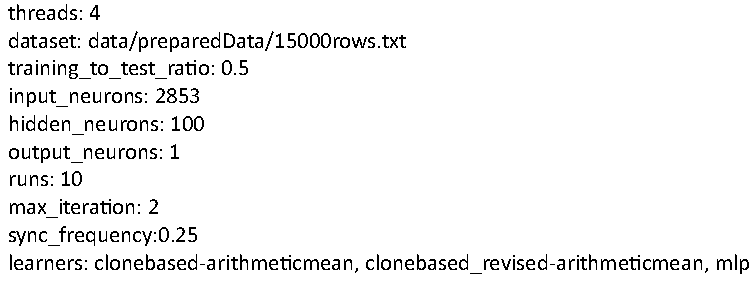
\includegraphics[scale=0.5]{Grafiken/testconfig}
		\end{center}
		\begin{center}	
			{\huge $\Downarrow$} {\small Evaluation}
		\end{center}
		\begin{center}
			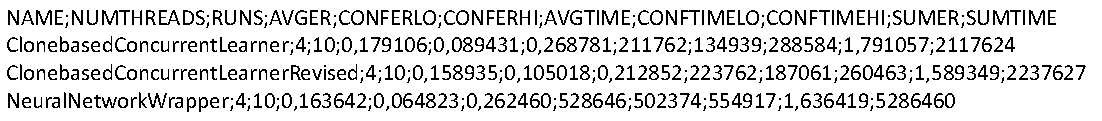
\includegraphics[scale=0.5]{Grafiken/csv}
			\newline
			\textbf{{\tiny Ergebnis als CSV}}
		\end{center}
	\end{frame}
	
	\subsection{Messwerte}
	\begin{frame}\frametitle{Aktuelle Evaluationswerte}
		\begin{block}{Experiment-Konfiguration}
			\begin{itemize}
				\item 5000 Datenreihen aus CERN-Satz, 1:1 Trainings-/Testdaten
				\item Intel Core2Quad Q6600, 4 Kerne à 2,4GHz, 8GB RAM
				\item JDK 7
			\end{itemize}
		\end{block}
		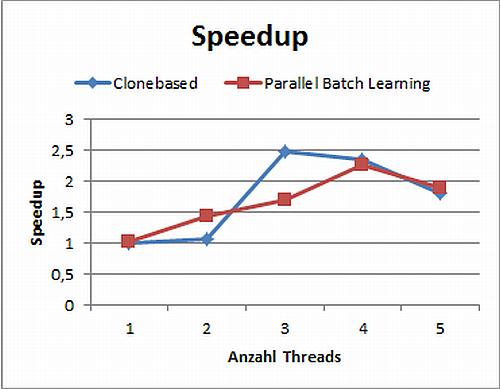
\includegraphics[width=0.51\textwidth]{images/eval_speedup.png}
		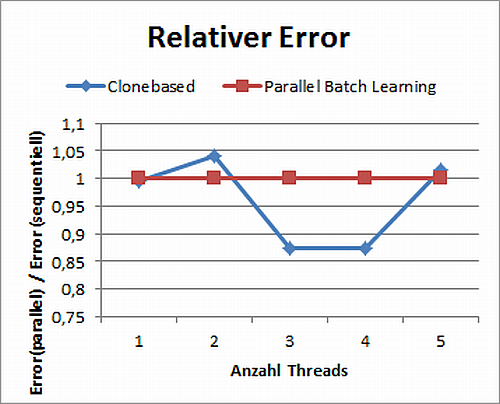
\includegraphics[width=0.49\textwidth]{images/eval_error.png}
	\end{frame}
	\section{Fazit}
	\subsection{Fazit}
	\begin{frame}\frametitle{Aktuelle Evaluationswerte}
		\textit{Klonen kann sich lohnen! (TODO)}
	\end{frame}

\end{document}

